%!TEX root = Slides.tex
\part{Anfragebearbeitung und Queryoptimierung}

\section{Einleitung}
\subsection{SQL-Anfragen}

\begin{frame}[fragile]{Grundlagen}
\framesubtitle{SQL-Anfragen}
\structure{SQL ist eine \textit{deskriptive} Sprache:}	
\begin{columns}
\begin{column}{.3\textwidth}
\begin{lstlisting}
 SELECT * FROM Kunde
 WHERE PLZ = 68165; 
\end{lstlisting}
\end{column}
	
\begin{column}{.58\textwidth}
\lstset{language=Java}
\begin{lstlisting}
 Vector result = new Vector(); 
  for (int i=0;i<kunden.size();i++) {
   Kunde tmpKunde = kunden.elementAt(i);
   if (tmpKunde.getPLZ()==68165) {
    result.add(tmpKunde);
   } 
  }
\end{lstlisting}
\end{column}
\end{columns}
\begin{itemize}
	\item SQL beschreibt das gewünschte Ergebnis. 
	\item Imperative Programmiersprache (Beispiel: Java) gibt Weg / Algorithmus an, wie Ergebnis berechnet wird.
	\item SQL-Anfragen entsprechen Termen in Relationaler Algebra. 
	\item In der Relationalen Algebra wird die Anwendungsreihenfolge der Operatoren beschrieben.
\end{itemize}
\end{frame}

\begin{frame}{Grundlagen}
\framesubtitle{SQL-Anfragen}
\structure{SQL-Ausführung auf der Datenbank}
\begin{itemize}
\item SQL-Abfrage wird vom Benutzer formuliert und an DBMS gesendet
\item DBMS nimmt Anfrage entgegen und muss entscheiden, wie Anfrage ausgeführt wird 
\item Ggf.~f\"uhrt DBMS Optimierung der Anfrage durch
\item Anfrage wird ausgeführt und Ergebnis zurückgegeben
\end{itemize}
\begin{block}{Beispiel (SQL und Relationale Algebra)}
\texttt{SELECT * from kunden NATURAL JOIN lieferungen WHERE KNR = 42}\\[4pt]
$\sigma_{kunden.knr=lieferungen.knr \wedge kunden.knr=42}(kunden\times lieferungen)$ 
\end{block}
%\alert{Die RA nimmt eine Zwischenstellung zwischen konkreter Berechnung und deskriptiver Beschreibung des Ergebnisses ein.}
\end{frame}

\subsection{Operatorbäume}

\begin{frame}{Grundlagen}
\framesubtitle{\insertsubsection}
\structure{DBMS übersetzt eine Anfrage in einen Operatorbaum}
\abs
\texttt{SELECT * from kunden NATURAL JOIN lieferungen WHERE KNR = 42}
\abs
\qtreecenterfalse
\begin{center}
\Tree[.$\sigma_{kunden.knr=lieferungen.knr \wedge knr=42}$ [.$\times$ \texttt{kunden} \texttt{lieferungen} ] ]
\end{center}
\begin{itemize}
\item Blätter eines Operatorbaums sind Operanden: Relationen oder Tupel-Variablen
\item Innere Knoten sind \textit{Operatoren}, die auf Ihre Kinder angewendet werden
\end{itemize}
\end{frame}

\begin{frame}{Grundlagen}
\framesubtitle{Operatorbäume}
\structure{Eine Anfrage kann mehrere mögliche Operatorbäume haben}
\abs
\texttt{SELECT * from kunden NATURAL JOIN lieferungen WHERE KNR = 42}
\abs
\begin{columns}
\begin{column}{.48\textwidth}
\qtreecenterfalse
\begin{center}\Tree[.$\sigma_{kunden.knr=lieferungen.knr \wedge knr=42}$ [.$\times$ \texttt{kunden} \texttt{lieferungen} ] ]
\end{center}	
\end{column}
\begin{column}{.48\textwidth}
	\qtreecenterfalse
	\begin{center}\Tree[.$\times$ [.$\sigma_{knr=42}$ \texttt{kunden} ] [.$\sigma_{knr=42}$ \texttt{lieferungen} ] ]
	\end{center}
\end{column}
\end{columns}
\vspace{1cm}
\alert{Welche Anfrage wird schneller ausgeführt?}
\abs
Grundsatz: Anfrageplan mit den geringsten Kosten soll ermittelt und ausgeführt werden.
\end{frame}

\subsection{Optimierung}
\begin{frame}{Grundlagen}
\framesubtitle{Parameter der Optimierung}
\structure{Optimaler Ausführungsplan abhängig von vielen Randbedingungen:}
\begin{itemize}
\item Blockgröße $b$
\item Puffergröße $mem$
\item Anzahl der Tupel der beteiligten Relationen (je Relation: $|r|$)
\item Anzahl der Blöcke, die Tupel aus den Relationen enthalten (je Relation: $b_r$)
\item Durchschnittliche Gr\"o\ss e eines Tupels (je Relation $r$: $size_r$)
\item Blocking Factor $bfr$
\item Anzahl unterschiedlicher Werte für ein Attribut $A$ einer Relation $r$: $val_{A,r}$
\item Anzahl der Ebenen eines Index-Baums f\"ur Attribut $A$ der Relation $r$: $lev_{I(R(A))}$
\item etc.
\end{itemize}
\end{frame}

\begin{frame}[t]{Grundlagen}
\framesubtitle{Parameter der Optimierung}
\structure{Einfache Metrik zur Berechnung der Kosten (Zeit von Platte zu Hauptspeicher):}
\begin{itemize}
\item $t_T$: Transferzeit eines Blocks 
\item $t_S$: Seek-Time f\"ur einen Block
\item $t_L$: Latency f\"ur Block-Sequenz
\end{itemize}
\abs
Kosten für $b$ Block-Transfers, $s$ Seeks, $\ell$ Latenzen: 
$$c = b \cdot t_T + s \cdot t_S + \ell t_L$$
\end{frame}

\begin{frame}{Grundlagen}
\framesubtitle{Operatorbäume}
\structure{Im Beispiel}
\\[4pt]
\texttt{SELECT * from kunden NATURAL JOIN lieferungen WHERE KNR = 42}
\abs
\begin{itemize}
\item Relationen \texttt{kunden} und \texttt{lieferungen} bestehen nur aus einem Datensatz:  
Beide Relationen vollständig mit jeweils einem Blockzugriff in den Hauptspeicher laden. Dort  
zum kartesischen Produkt aufbauen. Danach Selektion mit geringem Aufwand.
\pause
\item Relationen bestehen aus Tausenden/Millionen von Datensätzen: Zuerst Selektionen je Relation ausführen, damit 
nur relevante Datensätze im kartesischen Produkt kombiniert werden.
\begin{itemize}
\item Sind Indizes vorhanden, können relevante Daten schnell identifiziert werden
\item Sind keine Indizes vorhanden, müssen die Relationen vollständig durchsucht werden
\end{itemize}
\end{itemize}
\abs
\pause
Operatoren der relationalen Algebra können auf unterschiedliche Arten implementiert werden.
\end{frame}

\begin{frame}{Grundlagen}
\framesubtitle{Ziel der Optimierung}
\structure{Möglichst schnelle Anfragebearbeitung}
\begin{itemize}
\item Wenig Blockzugriffe bei Anfragebearbeitung, um Seektime und Latency zu minimieren 
\pause
\item In allen Operationen so wenig wie möglich Tupel verarbeiten 
\begin{itemize}
\item Selektionen so früh wie möglich durchf\"uhren
\item Basisoperationen nach Möglichkeit ohne Zwischenspeicherung von Teilergebnissen
\item Nur diejenigen Berechnungen durchführen, die Beitrag zur Bestimmung des Gesamtergebnisses haben. 
\item Keine redundanten Operationen oder leeren Ergebnismengen verarbeiten! 
\item Zusammenfassung gleicher Teilausdrücke für Wiederverwendung
\end{itemize}
\end{itemize}
\pause
Algorithmen, die im Hauptspeicher arbeiten, sollten effizient implementiert sein, können aber bei Kostensch\"atzung
meist vernachlässigt werden. 
\nl
Blockoperationen sind um Vielfaches aufwändiger.
\end{frame}

\section{Operationen}
\subsection{Scans}

\begin{frame}{Operationen}
\framesubtitle{Scans}
\structure{Scan ist eine der wesentlichen Operationen in einem DBMS}
\begin{itemize}
\item Er durchläuft alle Tupel einer Relation
\item Entspricht dem Arbeiten mit einem Cursor auf einer 'inneren' Datenbank- bzw. Dateiebene
\item Selektion und Projektion sind spezielle Scans
\end{itemize}
\pause
\abs
\structure{Aufteilung des Scans:}
\begin{itemize}
\item Full Table Scan durchläuft alle Tupel einer Relation in beliebiger Reihenfolge. 
\begin{itemize}
	\item Die Reihenfolge selbst wird dabei durch die Verteilung der Tupel auf Blöcke und ggf.~durch Pufferstrategie beeinflusst. 
	\item Es werden $b_r$ Operationen benötigt (Anzahl Blöcke, die Tupel Relation $r$ enthalten).
\end{itemize}
\item Index-Scan nutzt Index zum Auslesen der Datens\"atze in Sortierreihenfolge. 
\begin{itemize}
	\item Aufwand wird durch Anzahl der Index-Zugriffe und Anzahl Ergebniss\"atze bestimmt.
\end{itemize}
\end{itemize}
\end{frame}

\begin{frame}[fragile]{Operationen}
\framesubtitle{Scans}
\structure{Scans in der Praxis}
\\[6pt]
Gegeben sei Relation 
\\[4pt]
\texttt{Kunden(\uline{Kundennummer}, Vorname, Nachname)}
\\[4pt]
Auf Attribut \texttt{Kundennummer} ist ein Index definiert.
\begin{columns}[b]
	\lstset{captionpos=b}
	\begin{column}{.48\textwidth}
	\begin{lstlisting}[caption=Full Table Scan, xleftmargin=2ex, label=lst:fulltable]
SELECT * 
FROM Kunden; 
	\end{lstlisting}
	\end{column}
	\begin{column}{.48\textwidth}
	\begin{lstlisting}[caption=Index Scan, label=lst:indexscan]
SELECT * 
FROM Kunden
ORDER BY Kundennummer ASC; 
		\end{lstlisting}
	\end{column}
\end{columns}
\pause
\begin{itemize}
	\item Anfrage in Listing \ref{lst:fulltable} ben\"otigt keine Ordnungsstruktur. Somit kann Full Table Scan durchgeführt werden, 
	der minimale Anzahl Blockzugriffe benötigt.
	\pause
	\item Anfrage in Listing \ref{lst:indexscan} soll anhand Kundennummer sortiert werden. 
	In diesem Fall kann mit entsprechend sortiertem Index auf die Daten zugegriffen werden. 
\end{itemize} 
\end{frame}

\begin{frame}[fragile]{Operationen}
\framesubtitle{Scans}
	\structure{Full Table Scan}
	\begin{itemize}
		\item Minimale Anzahl von Blockzugriffen zum Auslesen der vollständigen Relation
		\item Ergebnisse ggf.~in unsortierter Reihenfolge 
		\item Es muss immer die vollständige Relation gelesen werden
	\end{itemize}
\pause
	\structure{Index Scan}
	\begin{itemize}
		\item Kann ggf.~Bereichsanfragen und Exact-Match-Anfragen bedienen 
		%\item Liefert die Datens\"atze unabhängig von der konkreten Blockbildung
		\item Liefert Bereichsanfrage mehr Datens\"atze als Gesamtzahl der Blöcke der Relation, kann 
		Full-Table-Scan mit expliziter Sortierung immer noch besser sein.
	\end{itemize}
%\alert{Für schreibende Operationen muss eine genaue Scan-Semantik eingehalten werden!}
\end{frame}

\begin{frame}[fragile]{Operationen}
\framesubtitle{Das Halloween-Problem}
\structure{Annahme: Die relevanten Datensätze für eine Update-Operation werden über Index-Scan 
	identifiziert. Im Beispiel: Index-Attribut \texttt{Preis}}
\abs
	\lstset{captionpos=b}
\begin{lstlisting}[xleftmargin=3ex,  label=lst:halloween]
UPDATE Produkt 
SET Preis = Preis * 1.1 
WHERE Preis < 100 ; 
\end{lstlisting}

\begin{enumerate}
\item Im Index wird an erste Position mit Preis $< 100$ gesprungen. 
\pause
\item Erster Datensatz wird geändert. 
\item Index wird geändert. Dadurch wandert der Datensatz an eine andere Position im Index/in der Datei, 
ist aber ggf.~immer noch $< 100$ (aber größer als bisher).
\pause
\item Im Index wird die nächste Position gesucht. Das kann dann wieder der gerade ge\"anderte Datensatz sein, der erneut geändert wird.
\end{enumerate}
\end{frame}

\begin{frame}[fragile]{Operationen}
\framesubtitle{Das Halloween-Problem}
\structure{Beim Halloween-Problem werden alle Datensätze so lange geändert, bis keiner mehr das Update-Krierium erfüllt.}
\pause
\begin{itemize}
\item Moderne DBMS sind gegen das Halloween-Problem resistent 
\item Der Index wird erst geändert, wenn alle betroffenen Datensätze geändert worden sind 
\end{itemize}
%\alert{Bei schreibenden Zugriffen ist die genaue Definition der Semantik des Schreibens wichtig! Auch wenn in DBMS dieses Problem weitgehend eliminiert worden ist, kann diese Information (ggf. auch in anderen Zusammenhängen) sinnvoll sein!}
\end{frame}

\begin{frame}[fragile]{Operationen}
\framesubtitle{Die Selektion}
\structure{Selektionen basieren im Allgemeinen auf Suchalgorithmen}
\begin{itemize}
	\item Jede Selektion kann \"uber Full Table Scan durchgeführt werden, um die Datensätze 
	{gem\"a\ss} der Selektionskriterien zu selektieren.
	\item Wenn ein geeigneter Index existiert, kann ein Index Scan durchgeführt werden.
	\pause
	\item Viele passende Suchalgorithmen und Mechanismen, um Selektion zu implementieren.
\end{itemize}

\end{frame}

\begin{frame}[fragile]{Operationen}
\framesubtitle{Die Selektion}
\structure{Brute Force Algorithmus}
\begin{itemize}
	\item Basiert auf dem Full Table Scan
	\pause
	\item Jeder Datensatz wird in den Hauptspeicher geladen.
	\pause
	\item Pr\"ufung im Hauptspeicher, ob Selektionskriterium erfüllt ist. 
	\pause
	\item Jeder Block wird in Hauptspeicher übertragen und linear durchsucht.
\end{itemize}
\abs
Brute Force Algorithmus funktioniert immer. 
\nl
Wird keine andere geeignete Implementierung gefunden, wird auf Brute Force zurückgegriffen. 
\end{frame}

\begin{frame}[fragile]{Operationen}
\framesubtitle{Die Selektion}
\structure{Binary Search Algorithmus}
\abs
\structure{Binary Search kann angewendet werden, wenn}
\begin{itemize}
	\item Selektiosbedingung eine Gleichheitsbedingung auf Schlüsselattribut ist 
	\item die Datendatei anhand dieses Attributs sortiert ist.
\end{itemize}
\abs
\begin{block}{Beispiel}
\texttt{SELECT * from Kunden WHERE Kundennummer = 1234}
\begin{itemize}
\item Kundennummer identifiziert jeden Kunden eindeutig
\item Sortierte Datendatei anhand der Kundennummer 
\end{itemize}
\end{block}
Damit sind die Kriterien erfüllt, um binäre Suche auf Datendatei durchzuführen. 
\nl 
Beachte: Es wurde kein Index verwendet.
\end{frame}

\begin{frame}[fragile]{Operationen}
\framesubtitle{Die Selektion}
\structure{Prim\"arindex}
\abs
\structure{Prim\"arindex / Hash-basierter Index kann angewendet werden, wenn}
\begin{itemize}
	\item Selektionsbedingung eine Gleichheitsbedingung ist  
	\item ein Primary Index bzw. Hash-basierter Index für das Attribut existiert
\end{itemize}
\abs
\begin{block}{Beispiel}
\texttt{SELECT * from Kunden WHERE Kundennummer = 1234}
\begin{itemize}
\item Annahme: Prim\"arindex / Hash-basierter Index auf \texttt{Kundennummer}
\end{itemize}
\end{block}
Damit sind die Kriterien erfüllt, um Suche über Prim\"arindex / Hash-basierten Index durchzuführen.
\end{frame}

\begin{frame}[fragile]{Operationen}
\framesubtitle{Die Selektion}
\structure{Prim\"arindex für Ungleichheitsoperationen}
\begin{itemize}
	\item Ist Selektionsbedingung eine Ungleichheitsbedingung auf Prim\"arindex-Attribut ($<, \leq, \neq, \geq, >$), 
	enthält die Ergebnismenge mehrere Einträge.
	\item Auch hier kann ggf. der Prim\"arindex verwendet werden.
\end{itemize}
\abs
\begin{block}{Beispiel}
\texttt{SELECT * from Produktgruppe WHERE prodGrID > 5}
\begin{itemize}
\item Annahme: Prim\"arindex auf \texttt{prodGrID}
\item Vorgehen: 
\begin{enumerate}
\item Finde Datensatz mit \texttt{prodGrID=5}.
\item Gib alle Nachfolger zurück.
\item Im Falle eines $<$ -- Operators: Gib alle Vorgänger zurück.
\end{enumerate}
\end{itemize}
\end{block}
\end{frame}

\begin{frame}[fragile]{Operationen}
\framesubtitle{Die Selektion}
\structure{B-B\"aume}
\begin{itemize}
\item Selektionsbedingung: Gleichheit auf (Nicht-)Schlüssel-Attribut. 
\item Selektionsbedingung: Ungleichheit
\begin{itemize}
\item Finde Datens\"atze mit Gleichheit.
\item Gib alle Nachfolger (f\"ur $>$) bzw.~Vorg\"anger (f\"ur $<$) zurück.
\end{itemize}
\end{itemize}
\abs
\begin{block}{Beispiel}
\texttt{SELECT * from Kunden WHERE PLZ [op] 68165}
\begin{itemize}
\item Annahme: B-Baum-Index auf PLZ
\item Index kann f\"ur Gleichheits- und Ungleichheitsabfragen verwendet werden: \texttt{[op]}: \texttt{<, >, =}
\end{itemize}
\end{block}
\end{frame}

\begin{frame}[fragile]{Operationen}
\framesubtitle{Die Selektion}
\structure{Beispiel}
\begin{itemize}
	\item Gegeben sei die Relation \texttt{Kunden(\uline{Kundennummer}, Vorname, Nachname)}
	\item Auf Attribut \texttt{Kundennummer} befindet sich ein Index -- prim\"ar oder sekund\"ar
\end{itemize}
\abs
Betrachte die folgenden Selektionen:
\begin{columns}
\lstset{captionpos=b}
\begin{column}{.48\textwidth}
\begin{lstlisting}[caption=Selektion \"uber Index-Feld, xleftmargin=3ex, label=lst:indexscan2]
SELECT * 
FROM Kunden
WHERE Kundennummer > 1000;
\end{lstlisting}
\end{column}	
\begin{column}{.48\textwidth}
\begin{lstlisting}[caption=Selektion \"uber Nicht-Index-Feld, label=lst:fulltable2]
SELECT * 
FROM Kunden
WHERE Nachname = 'Schmidt'; 
\end{lstlisting}
\end{column}
\end{columns}
\begin{itemize}
	\item Anfrage in Listing \ref{lst:indexscan2} über Index Scan effizienter -- obwohl vielleicht nicht auf 
	Sortierung in den Datens\"atzen zurückgegriffen werden kann --, da Bereich im Index eingrenzbar. 
	\item Anfrage in Listing \ref{lst:fulltable2} \"uber Full Table Scan, da kein Index ausgenutzt werden kann.
\end{itemize}
\end{frame}

\begin{frame}[fragile]{Operationen}
\framesubtitle{Verknüpfte Selektionsbedingungen}
\structure{Konjunktive Verknüpfungen mit einem Index}
\begin{block}{Beispiel}
\texttt{SELECT * from Kunde WHERE PLZ = 68165 AND Name = 'Meier'}
\begin{itemize}
	\item Besitzt \textit{ein} Attribut der Selektionsbedingung einen Zugriffsweg, wodurch schnelle 
	Selektion möglich ist, wird dieser verwendet.
	\item Das Ergebnis wird dann gegen die verbleibenden Bedingungen geprüft. 
	\item Existiert ein Kompositindex, wird dieser verwendet.
\end{itemize}
\end{block}
\end{frame}

\begin{frame}[fragile]{Operationen}
\framesubtitle{Verknüpfte Selektionsbedingungen}
\structure{Konjunktive Verknüpfungen mit einem Index}
\begin{columns}
\begin{column}{.60\textwidth}
\begin{figure}
\begin{tikzpicture}
\pie[sum=auto, radius=1.4, style=drop shadow] {10/68165, 100/}
\node[draw] at (0,-2.5) {\small{Alle PLZ}}; 
\draw[->] (2,0) -- (3,0);
\pie[sum=auto, radius=1.4, pos={5,0}, style=drop shadow] {2/Meier, 8/}
\node[draw] at (5,-2.5) {\small PLZ=68165}; 
\end{tikzpicture}
\end{figure}
\end{column}
\begin{column}{.37\textwidth}
\begin{enumerate}
\item Alle Datens\"atze mit \texttt{PLZ = 68165} werden über Index gesucht 
\item In der Ergebnismenge werden im Hauptspeicher ggf.~mit Nachladen alle Eintr\"age mit \texttt{Namen = 'Meier'} gesucht
\end{enumerate}
\end{column}
\end{columns}
\end{frame}

\begin{frame}[fragile]{Operationen}
\framesubtitle{Verknüpfte Selektionsbedingungen}
\structure{Konjunktive Verknüpfungen mit mehreren Indizes}
\abs
\begin{itemize}
	\item Es existieren für mehr als ein Attribut in der Konjunktion Indizes
	\item Ergebnis: Die Schnittmenge der Pointer / Bl\"ocke
\end{itemize}
\begin{figure}
  \def\firstcircle{(0,0) circle (1.5cm)}
  \def\secondcircle{(0:2cm) circle (1.5cm)}
  \colorlet{circle edge}{blue!50}
  \colorlet{circle area}{blue!20}    
  \tikzset{filled/.style={fill=circle area, draw=circle edge, thick}, outline/.style={draw=circle edge, thick}}    
  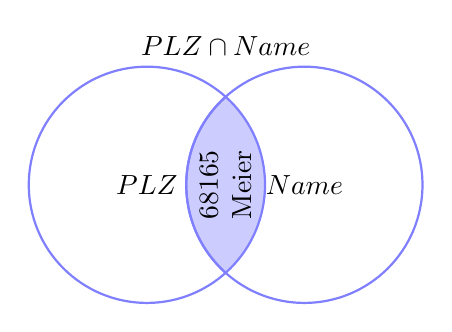
\begin{tikzpicture}
    \begin{scope}
        \clip \firstcircle;
        \fill[filled] \secondcircle;
    \end{scope}
    \draw[outline] \firstcircle node {$PLZ$};
    \draw[outline] \secondcircle node {$Name$};
    \node[anchor=south] at (current bounding box.north) {$PLZ \cap Name$};
    \node[rectangle, rotate=90,align=center] at (1,0){68165\\Meier}; 
  \end{tikzpicture}
\end{figure}
\end{frame}

\begin{frame}[fragile]{Operationen}
\framesubtitle{Verknüpfte Selektionsbedingungen}
\structure{Disjunktive Verknüpfungen}
\begin{block}{Beispiel}
\texttt{SELECT * from Kunde WHERE PLZ = 68165 OR Name = 'Meier'}
\end{block}
\begin{itemize}
	\item Optimierung der Disjunktion wesentlich schwieriger
	\item Ergebnismenge der Disjunktion ist Vereinigungsmenge (UNION) aller Teilergebnisse 
	\item Sobald nur ein einziges Attribut der Disjunktion keinen Zugriffspfad über Index besitzt, wird 
	Brute Force Ansatz (Full Table Scan) verwendet
\end{itemize}
\end{frame}

\begin{frame}[fragile]{Operationen}
\framesubtitle{Die Selektion}
\structure{Zusammenfassung}
\begin{itemize}
	\item Jedes DBMS hat mindestens die genannten Möglichkeiten, Selektionen zu optimieren. 
	\item \emph{Query Optimizer} wählt eine geeignete Strategie für die Ausführung aus -- komplexe Algorithmik!
	\item Auswahl erfolgt unter anderem anhand von Metadaten, die im Database Catalog gespeichert sind: 
	\begin{itemize}
		\item Anzahl der Tupel in einer Relation 
		\item Koeffizient für die geschätzte Anzahl von Tupeln, die einer Bedingung entsprechen (Selectivity $sel$)		
		\nl
		$\Rightarrow$ Gesch\"atzte Anzahl von Tupeln f\"ur eine Selektionsbedingung: $|r|\cdot sel$				
		%		\begin{itemize}
		%			%\item $ sel = \frac{1}{|r|}\text{\ bei Schl\"usselfeldern} $, $ sel = \frac{\frac{|r|}{i}}{|r|} \text{\ bei Nicht-Schl\"usselfeldern}$
		%			\item Gesch\"atzte Anzahl von Tupeln f\"ur eine Selektionsbedingung: $|r|\cdot sel$
		%		\end{itemize}
		\item etc. 
	\end{itemize}
\end{itemize}
\end{frame}

\subsection{Joins}

\begin{frame}[fragile]{Operationen}
\framesubtitle{Joins}
\structure{Eigenschaften von Joins}
\begin{itemize}
\item Optimierung ist sehr zeitintensiv
\item Joins werden in zwei Gruppen untergliedert: 
\begin{enumerate}
	\item Two-Way-Joins bilden einen Verbund von zwei Relationen
	\item Multi-Way-Joins bilden einen Verbund von mehr als zwei Relationen
\end{enumerate}
\pause
\item Zur Vereinfachung: Im Folgenden nur Two-Way Equi-Joins bzw.~Natural Joins 
%\item Zur Vereinfachung: Weitere Betrachtung beschränkt auf Two-Way-Joins, 
%da ansonsten die kombinatorische Anzahl an Ausführungsstrategien und Optimierungsmöglichkeiten zu groß wäre.
\end{itemize}
\end{frame}


\begin{frame}[fragile]{Operationen}
\framesubtitle{Joins}
\structure{Nested Loop Joins}
\begin{itemize}
	\item Basieren auf Brute Force Algorithmus 
	\item Benötigen keine speziellen Zugriffspfade in eine Datei
\end{itemize}
\pause
\abs
Vorgehen: 
			\lstset{ %this is the stype
				       % frame=tB,
				numbers=left, 
				numberstyle=\tiny,
				basicstyle=\scriptsize, 
				keywordstyle=\color{black}\bfseries,
				keywords={,input, output, return, datatype, function, in, if, else, foreach, while, begin, end, } %add the keywords you want, or load a language as Rubens explains in his comment above.
				numbers=left,
				xleftmargin=.03\textwidth,
			}			
\begin{lstlisting}
foreach r in R 
   foreach s in S 
      if r[JoinAttr] = s[JoinAttr]
         results.add(r.concat(s)); 
\end{lstlisting}
\pause
\textbf{Block-I/O-Laufzeitverhalten:} $\mathcal{O}(|R|\cdot |S|)$. Warum?
%Bessere Variante: Single Loop Join.
\end{frame}

\begin{frame}[fragile]{Operationen}
\framesubtitle{Joins}
\structure{Indexed Nested Loop Joins}
\begin{itemize}
	\item Innere Loop-Relation mit Index versehen\\[4pt]
\end{itemize}
\pause
Vorgehen:
\lstset{ %this is the stype
	%		  frame=tB,
	numbers=left, 
	numberstyle=\tiny,
	basicstyle=\scriptsize, 
	keywordstyle=\color{black}\bfseries,
	keywords={,input, output, return, datatype, function, in, if, else, foreach, while, begin, end, } %add the keywords you want, or load a language as Rubens explains in his comment above.
	numbers=left,
	xleftmargin=.04\textwidth,
}
\begin{lstlisting}
foreach r in R {
 tmpResult = S.indexLookup(r[JoinAttr]);
 foreach s in tmpResult 
  results.add(r.concat(s)); 
}
\end{lstlisting}
\pause
Gesamtkostenschätzung: $b_r(t_T+t_S+t_L)+n_r \cdot c $ 
\begin{itemize}
	\item $b_r$: Anzahl der Datenblöcke von Relation $R$
	\item $t_T + t_S + t_L$: Transfer Time, Seek Time, Latency 
	\item $n_r$: Anzahl Datens\"atze in $R$ 
	\item $c(|S|)$: Kosten für Einzelselektion aus S -- h\"angt von Gr\"o\ss e der Relation $S$ ab
\end{itemize}
\pause
\textbf{Block-I/O-Laufzeitverhalten:} $\mathcal{O}(|R|\cdot c(|S|))$. Warum?
\end{frame}

%\begin{frame}[fragile]{Operationen}
%\framesubtitle{Joins}
%\structure{Sort-Merge-Joins auf indizierten Relationen:}
%\begin{itemize}
%\item Sollten die Einträge zweier Relationen $R$ und $S$ physisch auf dem Join-Attribut sortiert sein, so kann das effiziente Sort-Merge-Join-Verfahren angewendet werden:
%\begin{itemize}
%\item Lese die Dateien für $R$ und $S$ \textit{gleichzeitig}
%\item Bilde den Verbund auf den einzelnen Tupeln, die der Join-Bedingung entsprechen
%\end{itemize}
%\item Sollten die Daten nicht sortiert vorliegen, können sie ggf. vorher durch einen externen Merge-Sort in eine Reihenfolge gebracht werden. 
%\end{itemize}
%\end{frame}

\begin{frame}
	\frametitle{Operationen}
	\framesubtitle{Joins}
	\structure{Hash Joins (für Natural Joins und Equi-Joins)}
	\abs
  Join der Relationen $R$ und $S$ auf den gemeinsamen Join-Attributen $\mathtt{[JoinAttrs]}$.
  \pause
  \abs
	Idee:
	\begin{itemize}
		\item Verwende Hashfunktion $h$ zur Partitionierung der Datens\"atze der beiden Relationen.
		\item Hash-Funktion partitioniert jede Relation auf den Join-Attributen $\mathtt{[JoinAttrs]}$.
		\item Nur noch die beiden Partitionen (Buckets) der beiden Relationen mit gleichem Hash-Wert werden jeweils 
		verglichen und ggf.~kombiniert.
	\end{itemize}	
\end{frame}

\begin{frame}
\frametitle{Operationen}
\framesubtitle{Joins}
\structure{Hash Joins (für Natural Joins und Equi-Joins)}
\abs
Arbeitsweise: 
\begin{itemize}
		\item Hash-Funktion $h$ bildet die Join-Attribute $\mathtt{[JoinAttrs]}$ der Relationen $R$ und $S$ auf die Werte 
		$\{0, 1, \dots, n\}$ ab.
		\pause
		\item $r_0, r_1, \dots, {r_n}$ bezeichnen die Partitionen/Buckets von Datens\"atzen aus $R$. 
		\item $s_0, s_1, \dots, {s_n}$ bezeichnen die Partitionen/Buckets von Datens\"atzen aus $S$. 
		\pause
		\item Jeder Datensatz $t_r \in R$ wird der Partition $r_i$ zugeordnet, mit $i = h(t_r\mathtt{[JoinAttrs]})$.
		\item Jeder Datensatz $t_s \in S$ wird der Partition $s_i$ zugeordnet, mit $i = h(t_s\mathtt{[JoinAttrs]})$.
		\pause
		\item M\"ogliche Verbundpartner in $R$ und $S$ sind somit auf gleiche Partitionsindizes abgebildet.
		\pause
		\item Nur noch Datens\"atze aus den Partitionen $r_i$ und $s_i$ m\"ussen vergleichen werden.
		\begin{itemize}
		 \item Vergleich notwendig, da Hash-Kollisionen vorkommen können.
		\end{itemize}
\end{itemize}	
\end{frame}

\begin{frame}[fragile]
	\frametitle{Operationen}
	\framesubtitle{Joins}
	\structure{Hash Joins (für Natural Joins und Equi-Joins)}
  \abs
	\structure{Vorgehen:}
			\lstset{ %this is the stype
	%		  frame=tB,
				numbers=left, 
				numberstyle=\tiny,
				basicstyle=\scriptsize, 
				keywordstyle=\color{black}\bfseries,
				keywords={,input, output, return, datatype, function, in, if, else, foreach, while, begin, end, } %add the keywords you want, or load a language as Rubens explains in his comment above.
				numbers=left,
				xleftmargin=.04\textwidth,
			}
\begin{lstlisting}
foreach r in R { 
   i = h(r[JoinAttr]);
   partitions[i].add(r);    
}
foreach s in S {
  i = h(s[JoinAttr]); 
  if (! partitions[i].isEmpty())
     foreach ri in partitions[i] 
        if (s[JoinAttr] == ri[JoinAttr])
           results.add(s.concat(ri));
}
\end{lstlisting}
\pause
\abs
Laufzeitverhalten: $\mathcal{O}([R]+ [S])$. Warum? 
\end{frame}

\section*{Übungsaufgaben}
\begin{frame}[t]
	\frametitle{\insertsection}
	
	\begin{alertblock}{Anfrageoptimierung}
		\begin{enumerate}
			\item Erläutern Sie den Zusammenhang zwischen SQL und der relationalen Algebra. Gehen Sie in Ihrer Antwort darauf ein, warum die relationale Algebra für die Anfrageauswertung benötigt wird und was ein Operatorbaum ist.
			\item Erläutern Sie anhand eines selbst gewählten Beispiels, warum die Operatoren der relationalen Algebra ggf. durch mehrere unterschiedliche Algorithmen in RDBMS implementiert werden.
			\item Erläutern Sie, warum eine Selektion mit disjunktiv verknüpften Bedingungen schwieriger zu optimieren ist als eine konjunktiv verknüpfte Selektionsbedingung.
			\item Eräutern Sie in eigenen Worten die Arbeitsweise eines Hash Joins.			
		\end{enumerate}
	\end{alertblock}
\end{frame}

%\subsection{Mengenoperationen}
%\begin{frame}[fragile]{Operationen}
%\framesubtitle{Mengenoperationen}
%\structure{Mengenoperationen können sehr effizient implementiert werden}
%\begin{itemize}
%\item Das kartesische Produkt sollte nach Möglichkeit nicht verwendet werden, da hier \textit{immer} der Brute %Force Ansatz verwendet wird. 
%\item Alle weiteren Mengenoperationen werden durch den Merge Sort Algorithmus implementiert. 
%\begin{itemize}
%\item Relationen werden nach dem gleichen Attribut sortiert
%\item Danach wird mit einem einzigen Scan das Ergebnis erzeugt. 
%\item Bsp. UNION: Beide Relationen werden zusammengefasst, doppelte Tupel werden nur einmal in das %Ergebnis eingebracht 
%\item Bsp. INTERSECT: Das Ergebnis beinhaltet nur diejenigen Tupel, die in beiden Relationen vorkommen
%\end{itemize}
%\end{itemize}
%\end{frame}
